\documentclass[11pt,aspectratio=169]{beamer}
\newcommand{\TalkShort}{Chapter 3, Sections 3.5.1--3.5.3}
% Visual reference: Matteo Di Sante, 13_06_26_slides_soaring_ctrw.tex.
% Steel-blue title bar, Palatino, Pisa seal, white pages and a pale title band.
\usepackage[T1]{fontenc}
\usepackage[utf8]{inputenc}
\usepackage[english]{babel}
\usepackage{mathpazo}
\usefonttheme{serif}
\usepackage{amsmath,amssymb,bm,booktabs,array,graphicx,tikz,microtype}
\usetikzlibrary{arrows.meta,calc,positioning}
\usepackage{siunitx}
\sisetup{group-separator={,},group-minimum-digits=4}
\usepackage{pgfpages}
\ifdefined\Speakernotes
  \setbeameroption{show notes on second screen=right}
\else
  \setbeameroption{hide notes}
\fi
\definecolor{pisablue}{RGB}{74,96,121}
\definecolor{pisablight}{RGB}{192,206,220}
\definecolor{accent}{RGB}{26,118,179}
\definecolor{para}{HTML}{3477A8}
\definecolor{hang}{HTML}{B5482A}
\definecolor{beginner}{HTML}{6A3D9A}
\definecolor{expert}{HTML}{C98A1E}
\definecolor{teal}{HTML}{2E7D8A}
\definecolor{wine}{HTML}{8E3B5C}
\definecolor{muted}{HTML}{666666}
\setbeamercolor{structure}{fg=pisablue}
\setbeamercolor{normal text}{fg=black,bg=white}
\setbeamercolor{frametitle}{fg=white,bg=pisablue}
\setbeamercolor{alerted text}{fg=accent}
\setbeamercolor{block title}{fg=white,bg=pisablue}
\setbeamercolor{block body}{fg=black,bg=pisablight!28}
\setbeamercolor{discussion}{fg=pisablue,bg=pisablight!30}
\setbeamercolor{button}{fg=white,bg=pisablue}
\setbeamerfont{button}{size=\normalsize}
\setbeamersize{text margin left=7mm,text margin right=7mm}
\setbeamertemplate{navigation symbols}{}
\setbeamertemplate{itemize item}{\textcolor{pisablue}{\small$\bullet$}}
\setbeamertemplate{itemize subitem}{\textcolor{pisablue}{\textendash}}
\setbeamertemplate{itemize/enumerate body begin}{\setlength{\itemsep}{0.55em}}
\setbeamertemplate{frametitle}{%
  \nointerlineskip
  \begin{beamercolorbox}[wd=\paperwidth,ht=9mm,dp=3mm,center]{frametitle}
    \large\insertframetitle\strut
  \end{beamercolorbox}
  \begin{tikzpicture}[remember picture,overlay]
    \node[anchor=north west,inner sep=0pt,xshift=2mm,yshift=-1.2mm]
      at(current page.north west){
\includegraphics[height=8mm]{assets/cherubino_white.png}};
    \node[anchor=north east,text=white,inner sep=0pt,xshift=-2.3mm,yshift=-4.2mm]
      at(current page.north east){\small\insertframenumber};
  \end{tikzpicture}
}
\setbeamertemplate{footline}{%
  \hspace{7mm}\textcolor{muted}{\fontsize{6.5}{8}\selectfont
    Matteo Di Sante\enspace|\enspace\TalkShort\enspace|\enspace13 September 2026}
  \hfill\textcolor{muted}{\fontsize{6.5}{8}\selectfont Supervisor discussion}\hspace{7mm}\vspace{2mm}
}
\newcommand{\kw}[1]{\textcolor{accent}{#1}}
\newcommand{\source}[1]{\par\vspace{1mm}{\fontsize{7}{8.3}\selectfont\color{muted}#1\par}}
\newcommand{\question}[1]{\par\vfill
  \begin{beamercolorbox}[wd=\linewidth,sep=5pt]{discussion}
    \small #1
  \end{beamercolorbox}}
\newcommand{\fig}[2][54mm]{\includegraphics[width=\linewidth,height=#1,keepaspectratio]{assets/#2}\par}
\newcommand{\speaker}[1]{\note{#1}}
\setbeamertemplate{note page}{%
  \vspace{4mm}\noindent%
  \begin{minipage}{\linewidth}
    {\small\color{pisablue}\TalkShort\quad|\quad Slide \insertframenumber}\par\medskip
    {\normalsize\bfseries\insertframetitle}\par\medskip
    {\small\insertnote}
  \end{minipage}
}
\newcommand{\refitem}[3]{\href{#1}{#2}\hfill {\color{muted}#3}\par\medskip}
\newcommand{\titleframe}[4]{%
\begin{frame}[plain]
\begin{tikzpicture}[remember picture,overlay]
 \fill[pisablue](current page.south west)rectangle(current page.north east);
 \fill[pisablight](current page.south west)rectangle([yshift=20mm]current page.south east);
 \node[anchor=north,yshift=-4mm]at(current page.north){
\includegraphics[height=13mm]{assets/cherubino_white.png}};
 \node[text=white,align=center]at([yshift=19mm]current page.center)
   {{\scshape\large University of Pisa}\\[2mm]{\small Department of Physics ``Enrico Fermi''}};
 \node[text=white,align=center,text width=.92\paperwidth]at([yshift=-3mm]current page.center)
   {{\LARGE\bfseries #1}\\[3mm]{\large #2}};
 \node[text=pisablue,align=center]at([yshift=10mm]current page.south)
   {{\normalsize Matteo Di Sante}\quad$\bullet$\quad{\normalsize 13 September 2026}\\[2mm]
    {\small #3}};
\end{tikzpicture}
\note{#4}
\end{frame}}
\newcommand{\backupstart}{%
\appendix
\begin{frame}[plain,noframenumbering]
\begin{tikzpicture}[remember picture,overlay]
 \fill[pisablue](current page.south west)rectangle(current page.north east);
 \node[text=white,align=center]at(current page.center)
  {{\LARGE\bfseries Discussion material}\\[4mm]{\large Extra figures, derivations and references}};
\end{tikzpicture}
\end{frame}}
\hypersetup{colorlinks=true,urlcolor=accent,linkcolor=accent,pdfauthor={Matteo Di Sante}}
% A notes sheet contains a second rendering of the slide. Disable its duplicate
% destinations; the normal slide PDF retains all hyperlinks and the viewer button.
\ifdefined\Speakernotes\hypersetup{draft}\fi

% Generated by scripts/reporting/ch3_global_transport/generate_revision_diagnostics.py -- do not edit.
\newcommand{\StatRevParaFlights}{155085}
\newcommand{\StatRevParaFixedFlights}{14360}
\newcommand{\StatRevParaLastFlights}{68207}
\newcommand{\StatRevParaLastWindows}{84997}
\newcommand{\StatRevParaLastOrderTwoFlights}{14360}
\newcommand{\StatRevParaAlphaOne}{1.703}
\newcommand{\StatRevParaAlphaTwo}{2.003}
\newcommand{\StatRevParaResidualOne}{0.050}
\newcommand{\StatRevParaResidualTwo}{0.071}
\newcommand{\StatRevParaFixedAlphaOne}{1.790}
\newcommand{\StatRevParaFixedAlphaTwo}{2.059}
\newcommand{\StatRevParaMomentZetaTwo}{1.737}
\newcommand{\StatRevParaMomentNuMin}{0.843}
\newcommand{\StatRevParaMomentNuMax}{0.883}
\newcommand{\StatRevParaMardiaMin}{-2.05}
\newcommand{\StatRevParaMardiaMedian}{0.67}
\newcommand{\StatRevParaMardiaMax}{5.91}
\newcommand{\StatRevParaOpenFlights}{67003}
\newcommand{\StatRevParaOpenAlphaOne}{1.770}
\newcommand{\StatRevParaOpenAlphaTwo}{1.937}
\newcommand{\StatRevParaOpenClosure}{0.365}
\newcommand{\StatRevParaClosedFlights}{87807}
\newcommand{\StatRevParaClosedAlphaOne}{1.623}
\newcommand{\StatRevParaClosedAlphaTwo}{2.036}
\newcommand{\StatRevParaClosedClosure}{0.027}
\newcommand{\StatRevParaEastLower}{0.811}
\newcommand{\StatRevParaEastMedian}{0.840}
\newcommand{\StatRevParaEastUpper}{0.844}
\newcommand{\StatRevParaEastNinetieth}{0.852}
\newcommand{\StatRevParaNorthLower}{0.837}
\newcommand{\StatRevParaNorthMedian}{0.858}
\newcommand{\StatRevParaNorthUpper}{0.863}
\newcommand{\StatRevParaNorthNinetieth}{0.878}
\newcommand{\StatRevParaRadialLower}{0.835}
\newcommand{\StatRevParaRadialMedian}{0.840}
\newcommand{\StatRevParaRadialUpper}{0.859}
\newcommand{\StatRevParaRadialNinetieth}{0.879}
\newcommand{\StatRevParaNarrowRadialLower}{0.975}
\newcommand{\StatRevParaNarrowRadialMedian}{0.895}
\newcommand{\StatRevParaNarrowRadialUpper}{0.862}
\newcommand{\StatRevParaNarrowRadialNinetieth}{0.872}
\newcommand{\StatRevParaQuantileFixedFlights}{14360}
\newcommand{\StatRevParaQuantileFixedOrigins}{21739115}
\newcommand{\StatRevParaQuantileControlFitMinS}{10}
\newcommand{\StatRevParaQuantileControlFitMaxS}{10000}
\newcommand{\StatRevParaQuantileChangingLower}{0.835}
\newcommand{\StatRevParaQuantileChangingMedian}{0.840}
\newcommand{\StatRevParaQuantileChangingUpper}{0.859}
\newcommand{\StatRevParaQuantileChangingNinetieth}{0.879}
\newcommand{\StatRevParaQuantileControlledLower}{0.976}
\newcommand{\StatRevParaQuantileControlledMedian}{0.899}
\newcommand{\StatRevParaQuantileControlledUpper}{0.890}
\newcommand{\StatRevParaQuantileControlledNinetieth}{0.898}
\newcommand{\StatRevParaDurationOneHFlights}{146786}
\newcommand{\StatRevParaDurationOneHRatio}{1.00}
\newcommand{\StatRevParaDurationTwoHFlights}{101980}
\newcommand{\StatRevParaDurationTwoHRatio}{1.09}
\newcommand{\StatRevParaDurationFourHFlights}{34594}
\newcommand{\StatRevParaDurationFourHRatio}{1.40}
\newcommand{\StatRevParaVacfTenAtSixHundred}{0.128}
\newcommand{\StatRevParaVacfSixtyAtSixHundred}{0.180}
\newcommand{\StatRevParaVacfThreeHundredAtSixHundred}{0.252}
\newcommand{\StatRevParaDurationReferenceLagS}{1070}
\newcommand{\StatRevHangFlights}{6060}
\newcommand{\StatRevHangFixedFlights}{563}
\newcommand{\StatRevHangLastFlights}{3313}
\newcommand{\StatRevHangLastWindows}{3920}
\newcommand{\StatRevHangLastOrderTwoFlights}{563}
\newcommand{\StatRevHangAlphaOne}{1.649}
\newcommand{\StatRevHangAlphaTwo}{1.985}
\newcommand{\StatRevHangResidualOne}{0.065}
\newcommand{\StatRevHangResidualTwo}{0.075}
\newcommand{\StatRevHangFixedAlphaOne}{1.744}
\newcommand{\StatRevHangFixedAlphaTwo}{2.025}
\newcommand{\StatRevHangMomentZetaTwo}{1.682}
\newcommand{\StatRevHangMomentNuMin}{0.832}
\newcommand{\StatRevHangMomentNuMax}{0.854}
\newcommand{\StatRevHangMardiaMin}{-1.64}
\newcommand{\StatRevHangMardiaMedian}{1.52}
\newcommand{\StatRevHangMardiaMax}{8.38}
\newcommand{\StatRevHangOpenFlights}{2183}
\newcommand{\StatRevHangOpenAlphaOne}{1.688}
\newcommand{\StatRevHangOpenAlphaTwo}{1.892}
\newcommand{\StatRevHangOpenClosure}{0.177}
\newcommand{\StatRevHangClosedFlights}{3877}
\newcommand{\StatRevHangClosedAlphaOne}{1.628}
\newcommand{\StatRevHangClosedAlphaTwo}{2.007}
\newcommand{\StatRevHangClosedClosure}{0.026}
\newcommand{\StatRevHangEastLower}{0.803}
\newcommand{\StatRevHangEastMedian}{0.806}
\newcommand{\StatRevHangEastUpper}{0.800}
\newcommand{\StatRevHangEastNinetieth}{0.817}
\newcommand{\StatRevHangNorthLower}{0.869}
\newcommand{\StatRevHangNorthMedian}{0.879}
\newcommand{\StatRevHangNorthUpper}{0.839}
\newcommand{\StatRevHangNorthNinetieth}{0.839}
\newcommand{\StatRevHangRadialLower}{0.860}
\newcommand{\StatRevHangRadialMedian}{0.829}
\newcommand{\StatRevHangRadialUpper}{0.821}
\newcommand{\StatRevHangRadialNinetieth}{0.845}
\newcommand{\StatRevHangNarrowRadialLower}{1.001}
\newcommand{\StatRevHangNarrowRadialMedian}{0.909}
\newcommand{\StatRevHangNarrowRadialUpper}{0.833}
\newcommand{\StatRevHangNarrowRadialNinetieth}{0.839}
\newcommand{\StatRevHangQuantileFixedFlights}{563}
\newcommand{\StatRevHangQuantileFixedOrigins}{791712}
\newcommand{\StatRevHangQuantileControlFitMinS}{10}
\newcommand{\StatRevHangQuantileControlFitMaxS}{10000}
\newcommand{\StatRevHangQuantileChangingLower}{0.860}
\newcommand{\StatRevHangQuantileChangingMedian}{0.829}
\newcommand{\StatRevHangQuantileChangingUpper}{0.821}
\newcommand{\StatRevHangQuantileChangingNinetieth}{0.845}
\newcommand{\StatRevHangQuantileControlledLower}{1.000}
\newcommand{\StatRevHangQuantileControlledMedian}{0.895}
\newcommand{\StatRevHangQuantileControlledUpper}{0.863}
\newcommand{\StatRevHangQuantileControlledNinetieth}{0.868}
\newcommand{\StatRevHangDurationOneHFlights}{5835}
\newcommand{\StatRevHangDurationOneHRatio}{1.01}
\newcommand{\StatRevHangDurationTwoHFlights}{4581}
\newcommand{\StatRevHangDurationTwoHRatio}{1.12}
\newcommand{\StatRevHangDurationFourHFlights}{1719}
\newcommand{\StatRevHangDurationFourHRatio}{1.50}
\newcommand{\StatRevHangVacfTenAtSixHundred}{0.124}
\newcommand{\StatRevHangVacfSixtyAtSixHundred}{0.173}
\newcommand{\StatRevHangVacfThreeHundredAtSixHundred}{0.249}
\newcommand{\StatRevHangDurationReferenceLagS}{1070}
\newcommand{\StatRevParaPcaReferenceLagS}{1000}
\newcommand{\StatRevParaPcaAlpsFlights}{90737}
\newcommand{\StatRevParaPcaAlpsRatio}{2.13}
\newcommand{\StatRevParaPcaAlpsAngle}{65.7}
\newcommand{\StatRevParaPcaPyreneesFlights}{12242}
\newcommand{\StatRevParaPcaPyreneesRatio}{2.19}
\newcommand{\StatRevParaPcaPyreneesAngle}{169.5}
\newcommand{\StatRevParaPcaChannelCoastFlights}{4890}
\newcommand{\StatRevParaPcaChannelCoastRatio}{1.92}
\newcommand{\StatRevParaPcaChannelCoastAngle}{29.7}
\newcommand{\StatRevHangPcaReferenceLagS}{1000}
\newcommand{\StatRevHangPcaAlpsFlights}{4535}
\newcommand{\StatRevHangPcaAlpsRatio}{1.55}
\newcommand{\StatRevHangPcaAlpsAngle}{85.0}
\newcommand{\StatRevHangPcaPyreneesFlights}{181}
\newcommand{\StatRevHangPcaPyreneesRatio}{1.68}
\newcommand{\StatRevHangPcaPyreneesAngle}{162.1}
\newcommand{\StatRevHangPcaChannelCoastFlights}{26}
\newcommand{\StatRevHangPcaChannelCoastRatio}{2.11}
\newcommand{\StatRevHangPcaChannelCoastAngle}{40.4}

% Generated by scripts/reporting/ch3_global_transport/generate_terrain_axis_comparison.py -- do not edit.
\newcommand{\StatTerrainAlpsAngle}{47.6}
\newcommand{\StatTerrainAlpsFlightAngle}{65.2}
\newcommand{\StatTerrainAlpsFlights}{46336}
\newcommand{\StatTerrainAlpsDifference}{17.6}
\newcommand{\StatTerrainAlpsMinAngle}{42.1}
\newcommand{\StatTerrainAlpsMaxAngle}{47.9}
\newcommand{\StatTerrainPyreneesAngle}{170.5}
\newcommand{\StatTerrainPyreneesFlightAngle}{170.5}
\newcommand{\StatTerrainPyreneesFlights}{4331}
\newcommand{\StatTerrainPyreneesDifference}{<1}
\newcommand{\StatTerrainPyreneesMinAngle}{169.7}
\newcommand{\StatTerrainPyreneesMaxAngle}{175.4}

% Generated by scripts/reporting/ch3_global_transport/generate_channel_wind_comparison.py -- do not edit.
\newcommand{\StatWindFlightAngle}{30.2}
\newcommand{\StatWindFlights}{1680}
\newcommand{\StatWindHeightM}{1006}
\newcommand{\StatWindHeightFlightM}{980}
\newcommand{\StatWindHeightLowM}{854}
\newcommand{\StatWindHeightHighM}{1160}
\newcommand{\StatWindWindows}{2013}
\newcommand{\StatWindSensitivityExcludedHours}{868}
\newcommand{\StatWindSensitivityAllLowAngle}{14.3}
\newcommand{\StatWindSensitivityAllHighAngle}{17.2}
\newcommand{\StatWindSensitivityDayLowAngle}{16.4}
\newcommand{\StatWindSensitivityDayHighAngle}{19.3}
\newcommand{\StatWindSurfaceAngle}{25.8}
\newcommand{\StatWindSurfaceFrom}{244.2}
\newcommand{\StatWindSurfaceDifference}{4.3}
\newcommand{\StatWindSurfaceResultant}{0.28}
\newcommand{\StatWindHundredAngle}{26.8}
\newcommand{\StatWindHundredFrom}{243.2}
\newcommand{\StatWindHundredDifference}{3.3}
\newcommand{\StatWindHundredResultant}{0.29}
\newcommand{\StatWindWarmDayAngle}{2.1}
\newcommand{\StatWindWarmDayFrom}{267.9}
\newcommand{\StatWindWarmDayDifference}{28.1}
\newcommand{\StatWindWarmDayResultant}{0.27}
\newcommand{\StatWindSurfaceDayAngle}{23.6}
\newcommand{\StatWindSurfaceDayFrom}{246.4}
\newcommand{\StatWindSurfaceDayDifference}{6.6}
\newcommand{\StatWindSurfaceDayResultant}{0.31}
\newcommand{\StatWindHundredDayAngle}{25.4}
\newcommand{\StatWindHundredDayFrom}{244.6}
\newcommand{\StatWindHundredDayDifference}{4.8}
\newcommand{\StatWindHundredDayResultant}{0.32}
\newcommand{\StatWindHeightAllAngle}{15.8}
\newcommand{\StatWindHeightAllFrom}{254.2}
\newcommand{\StatWindHeightAllDifference}{14.4}
\newcommand{\StatWindHeightAllResultant}{0.43}
\newcommand{\StatWindHeightDayAngle}{17.9}
\newcommand{\StatWindHeightDayFrom}{252.1}
\newcommand{\StatWindHeightDayDifference}{12.3}
\newcommand{\StatWindHeightDayResultant}{0.44}
\newcommand{\StatWindHeightWarmAllAngle}{16.0}
\newcommand{\StatWindHeightWarmAllFrom}{254.0}
\newcommand{\StatWindHeightWarmAllDifference}{14.2}
\newcommand{\StatWindHeightWarmAllResultant}{0.35}
\newcommand{\StatWindHeightWarmDayAngle}{20.6}
\newcommand{\StatWindHeightWarmDayFrom}{249.4}
\newcommand{\StatWindHeightWarmDayDifference}{9.6}
\newcommand{\StatWindHeightWarmDayResultant}{0.37}

% Generated by scripts/reporting/ch3_global_transport/generate_kinematic_isotropy_figure.py -- do not edit.
\newcommand{\StatKinFitMinS}{10}
\newcommand{\StatKinFitMaxS}{10000}
\newcommand{\StatKinMinFlights}{30}
\newcommand{\StatKinMinClusters}{10}
\newcommand{\StatKinParaFlights}{156406}
\newcommand{\StatKinParaPositionMedian}{0.82}
\newcommand{\StatKinParaPositionMin}{0.72}
\newcommand{\StatKinParaPositionMax}{0.87}
\newcommand{\StatKinParaVelocityMedian}{0.89}
\newcommand{\StatKinParaVelocityMin}{0.84}
\newcommand{\StatKinParaVelocityMax}{0.95}
\newcommand{\StatKinParaAccelerationMedian}{0.97}
\newcommand{\StatKinParaAccelerationMin}{0.95}
\newcommand{\StatKinParaAccelerationMax}{0.99}
\newcommand{\StatKinTerrainAlpsFlights}{91932}
\newcommand{\StatKinTerrainAlpsPositionMedian}{0.67}
\newcommand{\StatKinTerrainAlpsPositionMin}{0.60}
\newcommand{\StatKinTerrainAlpsPositionMax}{0.83}
\newcommand{\StatKinTerrainAlpsVelocityMedian}{0.81}
\newcommand{\StatKinTerrainAlpsVelocityMin}{0.68}
\newcommand{\StatKinTerrainAlpsVelocityMax}{0.92}
\newcommand{\StatKinTerrainAlpsAccelerationMedian}{0.97}
\newcommand{\StatKinTerrainAlpsAccelerationMin}{0.94}
\newcommand{\StatKinTerrainAlpsAccelerationMax}{1.00}
\newcommand{\StatKinTerrainAlpsEquipmentABFlights}{36605}
\newcommand{\StatKinTerrainAlpsEquipmentABPositionMedian}{0.61}
\newcommand{\StatKinTerrainAlpsEquipmentABPositionMin}{0.53}
\newcommand{\StatKinTerrainAlpsEquipmentABPositionMax}{0.75}
\newcommand{\StatKinTerrainAlpsEquipmentABVelocityMedian}{0.79}
\newcommand{\StatKinTerrainAlpsEquipmentABVelocityMin}{0.63}
\newcommand{\StatKinTerrainAlpsEquipmentABVelocityMax}{0.86}
\newcommand{\StatKinTerrainAlpsEquipmentABAccelerationMedian}{0.96}
\newcommand{\StatKinTerrainAlpsEquipmentABAccelerationMin}{0.91}
\newcommand{\StatKinTerrainAlpsEquipmentABAccelerationMax}{1.02}
\newcommand{\StatKinTerrainAlpsEquipmentCDCCCFlights}{51358}
\newcommand{\StatKinTerrainAlpsEquipmentCDCCCPositionMedian}{0.70}
\newcommand{\StatKinTerrainAlpsEquipmentCDCCCPositionMin}{0.62}
\newcommand{\StatKinTerrainAlpsEquipmentCDCCCPositionMax}{0.89}
\newcommand{\StatKinTerrainAlpsEquipmentCDCCCVelocityMedian}{0.83}
\newcommand{\StatKinTerrainAlpsEquipmentCDCCCVelocityMin}{0.71}
\newcommand{\StatKinTerrainAlpsEquipmentCDCCCVelocityMax}{0.97}
\newcommand{\StatKinTerrainAlpsEquipmentCDCCCAccelerationMedian}{0.97}
\newcommand{\StatKinTerrainAlpsEquipmentCDCCCAccelerationMin}{0.93}
\newcommand{\StatKinTerrainAlpsEquipmentCDCCCAccelerationMax}{1.01}
\newcommand{\StatKinTerrainPyreneesFlights}{12330}
\newcommand{\StatKinTerrainPyreneesPositionMedian}{1.67}
\newcommand{\StatKinTerrainPyreneesPositionMin}{1.21}
\newcommand{\StatKinTerrainPyreneesPositionMax}{5.05}
\newcommand{\StatKinTerrainPyreneesVelocityMedian}{1.19}
\newcommand{\StatKinTerrainPyreneesVelocityMin}{1.00}
\newcommand{\StatKinTerrainPyreneesVelocityMax}{1.39}
\newcommand{\StatKinTerrainPyreneesAccelerationMedian}{0.99}
\newcommand{\StatKinTerrainPyreneesAccelerationMin}{0.91}
\newcommand{\StatKinTerrainPyreneesAccelerationMax}{1.07}
\newcommand{\StatKinTerrainPyreneesEquipmentABFlights}{3971}
\newcommand{\StatKinTerrainPyreneesEquipmentABPositionMedian}{1.78}
\newcommand{\StatKinTerrainPyreneesEquipmentABPositionMin}{1.12}
\newcommand{\StatKinTerrainPyreneesEquipmentABPositionMax}{5.05}
\newcommand{\StatKinTerrainPyreneesEquipmentABVelocityMedian}{1.13}
\newcommand{\StatKinTerrainPyreneesEquipmentABVelocityMin}{0.98}
\newcommand{\StatKinTerrainPyreneesEquipmentABVelocityMax}{1.50}
\newcommand{\StatKinTerrainPyreneesEquipmentABAccelerationMedian}{0.98}
\newcommand{\StatKinTerrainPyreneesEquipmentABAccelerationMin}{0.89}
\newcommand{\StatKinTerrainPyreneesEquipmentABAccelerationMax}{1.08}
\newcommand{\StatKinTerrainPyreneesEquipmentCDCCCFlights}{7964}
\newcommand{\StatKinTerrainPyreneesEquipmentCDCCCPositionMedian}{1.60}
\newcommand{\StatKinTerrainPyreneesEquipmentCDCCCPositionMin}{1.22}
\newcommand{\StatKinTerrainPyreneesEquipmentCDCCCPositionMax}{5.11}
\newcommand{\StatKinTerrainPyreneesEquipmentCDCCCVelocityMedian}{1.20}
\newcommand{\StatKinTerrainPyreneesEquipmentCDCCCVelocityMin}{1.01}
\newcommand{\StatKinTerrainPyreneesEquipmentCDCCCVelocityMax}{1.35}
\newcommand{\StatKinTerrainPyreneesEquipmentCDCCCAccelerationMedian}{0.99}
\newcommand{\StatKinTerrainPyreneesEquipmentCDCCCAccelerationMin}{0.92}
\newcommand{\StatKinTerrainPyreneesEquipmentCDCCCAccelerationMax}{1.07}
\newcommand{\StatKinTerrainChannelCoastFlights}{4963}
\newcommand{\StatKinTerrainChannelCoastPositionMedian}{0.96}
\newcommand{\StatKinTerrainChannelCoastPositionMin}{0.89}
\newcommand{\StatKinTerrainChannelCoastPositionMax}{1.09}
\newcommand{\StatKinTerrainChannelCoastVelocityMedian}{0.97}
\newcommand{\StatKinTerrainChannelCoastVelocityMin}{0.90}
\newcommand{\StatKinTerrainChannelCoastVelocityMax}{1.11}
\newcommand{\StatKinTerrainChannelCoastAccelerationMedian}{0.97}
\newcommand{\StatKinTerrainChannelCoastAccelerationMin}{0.88}
\newcommand{\StatKinTerrainChannelCoastAccelerationMax}{1.07}
\newcommand{\StatKinTerrainChannelCoastEquipmentABFlights}{879}
\newcommand{\StatKinTerrainChannelCoastEquipmentABPositionMedian}{1.12}
\newcommand{\StatKinTerrainChannelCoastEquipmentABPositionMin}{0.76}
\newcommand{\StatKinTerrainChannelCoastEquipmentABPositionMax}{1.75}
\newcommand{\StatKinTerrainChannelCoastEquipmentABVelocityMedian}{0.97}
\newcommand{\StatKinTerrainChannelCoastEquipmentABVelocityMin}{0.74}
\newcommand{\StatKinTerrainChannelCoastEquipmentABVelocityMax}{1.38}
\newcommand{\StatKinTerrainChannelCoastEquipmentABAccelerationMedian}{0.96}
\newcommand{\StatKinTerrainChannelCoastEquipmentABAccelerationMin}{0.72}
\newcommand{\StatKinTerrainChannelCoastEquipmentABAccelerationMax}{1.20}
\newcommand{\StatKinTerrainChannelCoastEquipmentCDCCCFlights}{3789}
\newcommand{\StatKinTerrainChannelCoastEquipmentCDCCCPositionMedian}{0.98}
\newcommand{\StatKinTerrainChannelCoastEquipmentCDCCCPositionMin}{0.92}
\newcommand{\StatKinTerrainChannelCoastEquipmentCDCCCPositionMax}{1.09}
\newcommand{\StatKinTerrainChannelCoastEquipmentCDCCCVelocityMedian}{0.98}
\newcommand{\StatKinTerrainChannelCoastEquipmentCDCCCVelocityMin}{0.90}
\newcommand{\StatKinTerrainChannelCoastEquipmentCDCCCVelocityMax}{1.10}
\newcommand{\StatKinTerrainChannelCoastEquipmentCDCCCAccelerationMedian}{0.97}
\newcommand{\StatKinTerrainChannelCoastEquipmentCDCCCAccelerationMin}{0.87}
\newcommand{\StatKinTerrainChannelCoastEquipmentCDCCCAccelerationMax}{1.10}
\newcommand{\StatKinEquipmentABFlights}{54574}
\newcommand{\StatKinEquipmentABPositionMedian}{0.74}
\newcommand{\StatKinEquipmentABPositionMin}{0.65}
\newcommand{\StatKinEquipmentABPositionMax}{0.80}
\newcommand{\StatKinEquipmentABVelocityMedian}{0.85}
\newcommand{\StatKinEquipmentABVelocityMin}{0.78}
\newcommand{\StatKinEquipmentABVelocityMax}{0.91}
\newcommand{\StatKinEquipmentABAccelerationMedian}{0.97}
\newcommand{\StatKinEquipmentABAccelerationMin}{0.93}
\newcommand{\StatKinEquipmentABAccelerationMax}{1.00}
\newcommand{\StatKinEquipmentCDCCCFlights}{95157}
\newcommand{\StatKinEquipmentCDCCCPositionMedian}{0.86}
\newcommand{\StatKinEquipmentCDCCCPositionMin}{0.74}
\newcommand{\StatKinEquipmentCDCCCPositionMax}{0.91}
\newcommand{\StatKinEquipmentCDCCCVelocityMedian}{0.91}
\newcommand{\StatKinEquipmentCDCCCVelocityMin}{0.86}
\newcommand{\StatKinEquipmentCDCCCVelocityMax}{0.97}
\newcommand{\StatKinEquipmentCDCCCAccelerationMedian}{0.98}
\newcommand{\StatKinEquipmentCDCCCAccelerationMin}{0.94}
\newcommand{\StatKinEquipmentCDCCCAccelerationMax}{1.00}
\newcommand{\StatKinHangFlights}{6094}
\newcommand{\StatKinHangPositionMedian}{1.03}
\newcommand{\StatKinHangPositionMin}{0.54}
\newcommand{\StatKinHangPositionMax}{1.45}
\newcommand{\StatKinHangVelocityMedian}{1.05}
\newcommand{\StatKinHangVelocityMin}{0.76}
\newcommand{\StatKinHangVelocityMax}{1.19}
\newcommand{\StatKinHangAccelerationMedian}{1.01}
\newcommand{\StatKinHangAccelerationMin}{0.86}
\newcommand{\StatKinHangAccelerationMax}{1.16}

% Generated by scripts/reporting/ch2_dataset/generate_prelim_figure.py -- do not edit.
\newcommand{\StatPrelimParaBelowCutFlights}{533}
\newcommand{\StatPrelimParaBelowCutPct}{0.34}
\newcommand{\StatPrelimParaFlights}{156449}
\newcommand{\StatPrelimParaMedianDurH}{2.63}
\newcommand{\StatPrelimParaMedianPathKm}{87}
\newcommand{\StatPrelimParaMedianFixes}{7138}
\newcommand{\StatPrelimParaMedianDtS}{1}
\newcommand{\StatPrelimParaOneHertzPct}{69.9}
\newcommand{\StatPrelimParaDurationIqrLowH}{1.77}
\newcommand{\StatPrelimParaDurationIqrHighH}{3.93}
\newcommand{\StatPrelimParaPathIqrLowKm}{57}
\newcommand{\StatPrelimParaPathIqrHighKm}{134}
\newcommand{\StatPrelimParaAbroadPct}{5.3}
\newcommand{\StatPrelimParaMetroFlights}{148119}
\newcommand{\StatPrelimParaMetroPct}{94.7}
\newcommand{\StatPrelimParaReunionFlights}{4949}
\newcommand{\StatPrelimParaReunionPct}{3.2}
\newcommand{\StatPrelimParaElsewhereFlights}{3381}
\newcommand{\StatPrelimParaElsewherePct}{2.2}
\newcommand{\StatPrelimParaGroupAlpsPct}{58.8}
\newcommand{\StatPrelimParaGroupPyreneesPct}{7.9}
\newcommand{\StatPrelimParaGroupMassifCentralPct}{8.2}
\newcommand{\StatPrelimParaGroupChannelCoastPct}{3.2}
\newcommand{\StatPrelimParaGroupOutsideMassifsPct}{16.7}
\newcommand{\StatPrelimParaSites}{5341}
\newcommand{\StatPrelimParaGroupAlpsAltMedianM}{1370}
\newcommand{\StatPrelimParaGroupAlpsAltNinetyPctM}{2017}
\newcommand{\StatPrelimParaGroupPyreneesAltMedianM}{1402}
\newcommand{\StatPrelimParaGroupPyreneesAltNinetyPctM}{1882}
\newcommand{\StatPrelimParaGroupMassifCentralAltMedianM}{933}
\newcommand{\StatPrelimParaGroupMassifCentralAltNinetyPctM}{1561}
\newcommand{\StatPrelimParaGroupChannelCoastAltMedianM}{220}
\newcommand{\StatPrelimParaGroupChannelCoastAltNinetyPctM}{417}
\newcommand{\StatPrelimParaIsoRatioMin}{0.70}
\newcommand{\StatPrelimParaIsoRatioMax}{0.86}
\newcommand{\StatPrelimParaIsoRatioMedian}{0.80}
\newcommand{\StatPrelimParaClassStrata}{6}
\newcommand{\StatPrelimParaClassMaxDeparturePct}{90}
\newcommand{\StatPrelimParaClassTypicalDeparturePct}{51}
\newcommand{\StatPrelimParaGroupStrata}{6}
\newcommand{\StatPrelimParaGroupMaxDeparturePct}{351}
\newcommand{\StatPrelimParaGroupTypicalDeparturePct}{71}
\newcommand{\StatPrelimParaSeasonStrata}{17}
\newcommand{\StatPrelimParaSeasonMaxDeparturePct}{21}
\newcommand{\StatPrelimParaSeasonTypicalDeparturePct}{12}
\newcommand{\StatPrelimHangBelowCutFlights}{9}
\newcommand{\StatPrelimHangBelowCutPct}{0.15}
\newcommand{\StatPrelimHangFlights}{6102}
\newcommand{\StatPrelimHangMedianDurH}{3.07}
\newcommand{\StatPrelimHangMedianPathKm}{151}
\newcommand{\StatPrelimHangMedianFixes}{3345}
\newcommand{\StatPrelimHangMedianDtS}{3}
\newcommand{\StatPrelimHangOneHertzPct}{28.0}
\newcommand{\StatPrelimHangDurationIqrLowH}{2.11}
\newcommand{\StatPrelimHangDurationIqrHighH}{4.29}
\newcommand{\StatPrelimHangPathIqrLowKm}{99}
\newcommand{\StatPrelimHangPathIqrHighKm}{225}
\newcommand{\StatPrelimHangAbroadPct}{3.3}
\newcommand{\StatPrelimHangMetroFlights}{5900}
\newcommand{\StatPrelimHangMetroPct}{96.7}
\newcommand{\StatPrelimHangReunionFlights}{7}
\newcommand{\StatPrelimHangReunionPct}{0.1}
\newcommand{\StatPrelimHangElsewhereFlights}{195}
\newcommand{\StatPrelimHangElsewherePct}{3.2}
\newcommand{\StatPrelimHangGroupAlpsPct}{75.0}
\newcommand{\StatPrelimHangGroupPyreneesPct}{3.0}
\newcommand{\StatPrelimHangGroupMassifCentralPct}{3.9}
\newcommand{\StatPrelimHangGroupChannelCoastPct}{0.4}
\newcommand{\StatPrelimHangGroupOutsideMassifsPct}{14.5}
\newcommand{\StatPrelimHangSites}{388}
\newcommand{\StatPrelimHangGroupAlpsAltMedianM}{1345}
\newcommand{\StatPrelimHangGroupAlpsAltNinetyPctM}{1566}
\newcommand{\StatPrelimHangGroupPyreneesAltMedianM}{1590}
\newcommand{\StatPrelimHangGroupPyreneesAltNinetyPctM}{2221}
\newcommand{\StatPrelimHangGroupMassifCentralAltMedianM}{876}
\newcommand{\StatPrelimHangGroupMassifCentralAltNinetyPctM}{1441}
\newcommand{\StatPrelimHangGroupChannelCoastAltMedianM}{181}
\newcommand{\StatPrelimHangGroupChannelCoastAltNinetyPctM}{236}
\newcommand{\StatPrelimHangIsoRatioMin}{0.54}
\newcommand{\StatPrelimHangIsoRatioMax}{1.44}
\newcommand{\StatPrelimHangIsoRatioMedian}{1.20}
\newcommand{\StatPrelimHangClassStrata}{1}
\newcommand{\StatPrelimHangClassMaxDeparturePct}{34}
\newcommand{\StatPrelimHangClassTypicalDeparturePct}{34}
\newcommand{\StatPrelimHangGroupStrata}{1}
\newcommand{\StatPrelimHangGroupMaxDeparturePct}{29}
\newcommand{\StatPrelimHangGroupTypicalDeparturePct}{29}
\newcommand{\StatPrelimMinStratum}{2000}
\newcommand{\StatPrelimIsoBootResamples}{200}

\hypersetup{pdftitle={Directional structure, terrain and equipment}}
\title{Directional structure, terrain and equipment}
\begin{document}
\titleframe{Directional structure, terrain and equipment}
 {Regional measurements and environmental interpretation}
 {Thesis Sections 3.5.1, 3.5.2 and 3.5.3}
 {The presentation follows the three thesis subsections in order, including every panel of Figures 3.20--3.26. Figures with several panels are followed by enlarged views.}
\section{East--north balance in the retained archive}
\subsectionframe{3.5.1}{East--north balance in the retained archive}

\begin{frame}{The ratio compares motion along east and north}
\[
 \rho_{EN}(t)=\frac{\langle E_f(t)^2\rangle_f}{\langle N_f(t)^2\rangle_f},
 \qquad
 \langle E_f^2\rangle_f=\operatorname{Var}_f(E_f)+\langle E_f\rangle_f^2.
\]
\small $E_f(t)$ and $N_f(t)$ are positions relative to launch. The clock is time
since launch; each time uses the flights that still contribute paired observations.
\par\medskip
$\rho_{EN}>1$: larger east second moment. \qquad
$\rho_{EN}<1$: larger north second moment.
\par\medskip
The ratio combines mean displacement and spread. Equality is one necessary
condition for isotropy; cross moments and the full angular distribution also matter.
\source{Thesis Section 3.5.1.}
\question{How much of the imbalance comes from mean motion, and how much from spread around the mean?}
\speaker{Launch-referenced positions may retain reacquisition offsets across missing intervals. The subsequent PCA uses increments wholly inside segments; these avoid crossing gaps but do not independently validate their endpoints.}
\end{frame}

\begin{frame}{The retained archive has unequal east and north moments}
\begin{columns}[c,onlytextwidth]
\column{.68\textwidth}
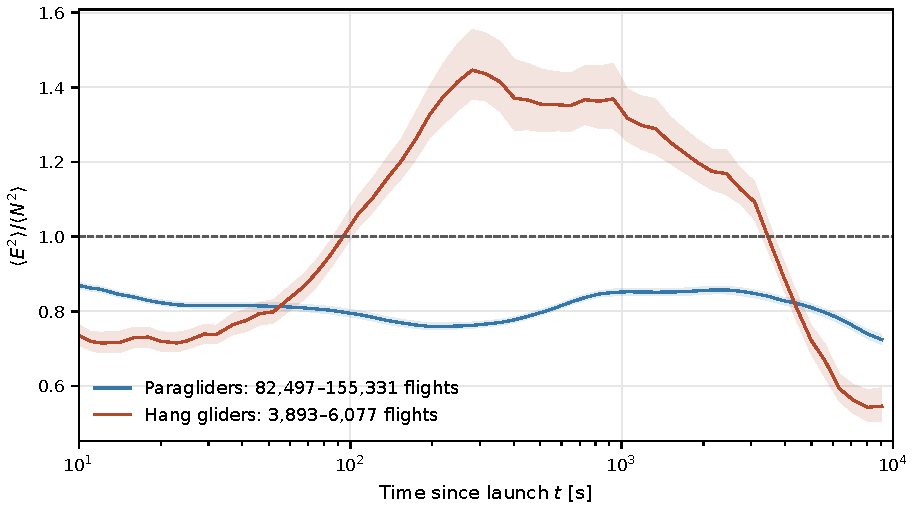
\includegraphics[width=\linewidth,height=53mm,keepaspectratio]{../thesis/generated/prelim_isotropy.pdf}
\column{.29\textwidth}\small
Curve ranges over 10--10,000 s:\par\medskip
Paragliders: \StatPrelimParaIsoRatioMin--\StatPrelimParaIsoRatioMax.\par\medskip
Hang gliders: \StatPrelimHangIsoRatioMin--\StatPrelimHangIsoRatioMax.\par\medskip
The paraglider curve stays below one. The hang-glider curve crosses it.
\end{columns}
\source{Thesis Fig. 3.20, complete figure. Numbers are extrema of the observed curves; shading is the bootstrap range.}
\question{Would a fixed population change the time dependence of either ratio?}
\speaker{The directional imbalance motivates studying east, north and radial displacement separately. Route choice, terrain, wind and selection can all contribute. The curve ranges are not limits of the uncertainty bands.}
\end{frame}

\begin{frame}{The bands resample whole take-off sites and days}
\small
A site--day groups flights with the same recorded take-off site and date.
Flights in one group may share weather and route conditions.
\begin{enumerate}
 \item Resample whole groups with replacement, keeping their flights together.
 \item Recompute the paired east/north moment ratio at every supported time.
 \item Repeat \StatPrelimIsoBootResamples\ times; retain the 10th and 90th percentiles.
\end{enumerate}
The shading contains the central 80\% of bootstrap estimates at each time.
Plots require \StatPrelimIsoMinFlights\ flights and
\StatPrelimIsoMinClusters\ contributing groups.
\source{Thesis Fig. 3.20 and the uncertainty convention used in Figs. 3.24--3.26.}
\question{How much dependence remains across nearby sites, successive days or repeated pilots?}
\speaker{These are pointwise ranges, not simultaneous bands or the spread of individual flights. Missing site/date keys become singleton groups. Resampling preserves observed within-group dependence; it assumes groups can be independently resampled. It does not match equipment groups on weather.}
\end{frame}

\section{Regional principal axes}
\subsectionframe{3.5.2}{Regional principal axes}

\begin{frame}{PCA measures spread around the mean displacement}
\[
 \mathbf X_f(t,\tau)=\mathbf r_f(t+\tau)-\mathbf r_f(t),\qquad
 \boldsymbol\mu_g=\langle\mathbf X\rangle_g,
\]
\[
 \Sigma_g(\tau)=\left\langle
 (\mathbf X-\boldsymbol\mu_g)(\mathbf X-\boldsymbol\mu_g)^\top
 \right\rangle_g
 =U_g\,\operatorname{diag}(\lambda_1,\lambda_2)\,U_g^\top.
\]
\small The leading eigenvector gives the axis of greatest spread;
$\lambda_1/\lambda_2$ measures covariance anisotropy.
\par\medskip
Use every supported increment in the regional archive on the 10-s grid.
Origins are spaced by the lag within each segment. Flights with more
origins receive more weight.
\source{Thesis Section 3.5.2. Lags: 10, 100, 1000 and 10,000 s.}
\question{Would equal flight weights or fixed membership change the regional axes?}
\speaker{No increment crosses a segment boundary. The available population can shrink with lag. Eight flights is the display minimum, not a precision guarantee. Angles run counterclockwise from east, modulo 180 degrees; they become poorly determined when the two eigenvalues are close.}
\end{frame}

\begin{frame}{The ellipses show shape and direction at four lags}
\begin{columns}[c,onlytextwidth]
\column{.55\textwidth}
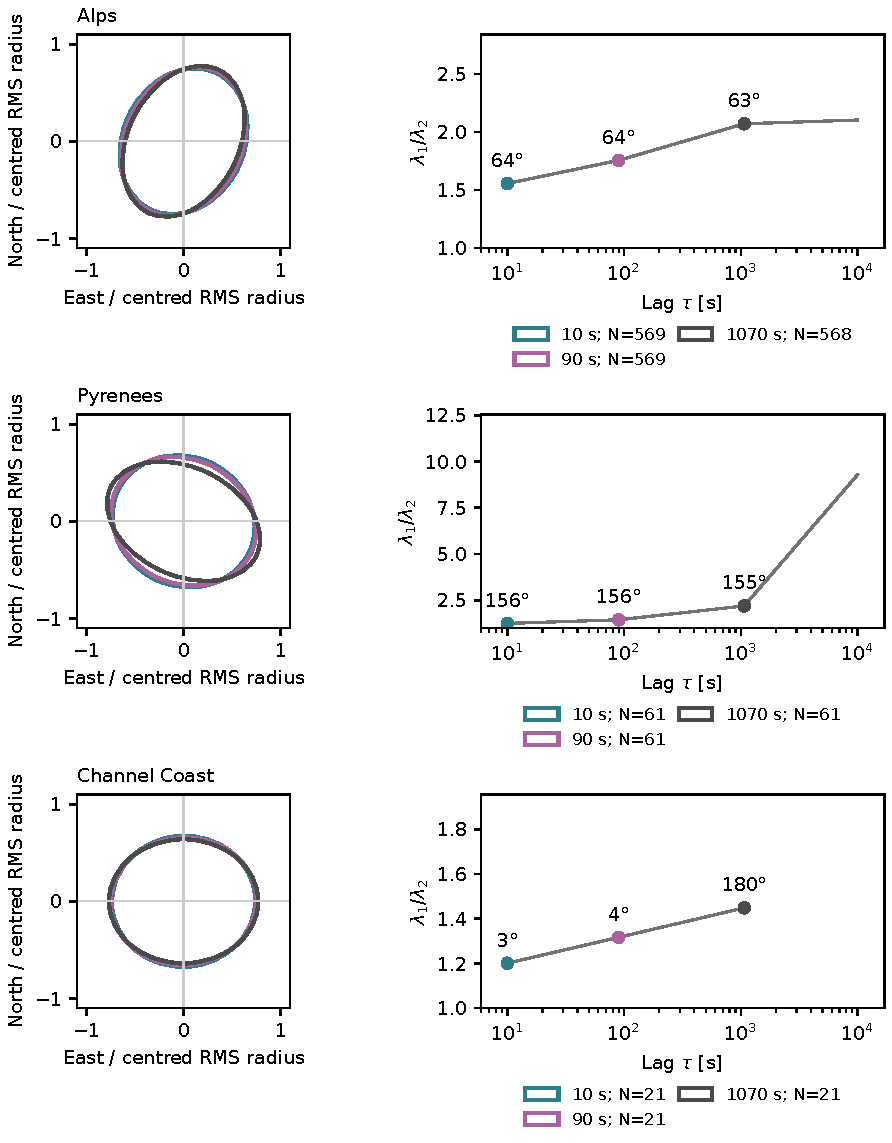
\includegraphics[width=\linewidth,height=57mm,keepaspectratio]{../thesis/generated/ch3_pca.pdf}
\column{.42\textwidth}\small
Both coordinates are divided by the same centred RMS radius:
\[
 s_g(\tau)=\sqrt{\operatorname{tr}\Sigma_g(\tau)}.
\]
\[
 \mathbf X^*=\frac{\mathbf X-\boldsymbol\mu_g}{s_g(\tau)}.
\]
Each region and lag has its own factor. Shape and angle are preserved;
absolute displacement amplitude is removed.
\end{columns}
\source{Thesis Fig. 3.21, all three rows. Right: eigenvalue ratio; labels give axis angles.}
\speaker{Normalising by one scalar preserves the eigenvalue ratio. This differs from whitening, which separately normalises the principal directions. The following slides enlarge the three original rows.}
\end{frame}

\begin{frame}{Alps: the principal axes change with lag}
\centering\fig[48mm]{section35-pca-alps.pdf}
\takeaway{At \StatRevParaPcaReferenceLagS\ s: $\lambda_1/\lambda_2=\StatRevParaPcaAlpsRatio$,
 axis \StatRevParaPcaAlpsAngle$^\circ$; \num{\StatRevParaPcaAlpsFlights} flights.}
\source{Thesis Fig. 3.21, original Alps row. Each ellipse uses its own centred RMS radius.}
\question{How much of the change follows route geometry, and how much follows the changing population?}
\speaker{The plotted axis is modulo 180 degrees. A nearly circular ellipse does not determine a precise preferred axis. Coastal take-offs do not provide an isotropic reference by definition.}
\end{frame}

\begin{frame}{Pyrenees: the principal axes change with lag}
\centering\fig[48mm]{section35-pca-pyrenees.pdf}
\takeaway{The axis approaches east--west and the eigenvalue ratio rises at long lag,
 while the contributing population falls.}
\source{Thesis Fig. 3.21, original Pyrenees row. Each ellipse uses its own centred RMS radius.}
\question{How much of the change follows route geometry, and how much follows the changing population?}
\speaker{The plotted axis is modulo 180 degrees. A nearly circular ellipse does not determine a precise preferred axis. Coastal take-offs do not provide an isotropic reference by definition.}
\end{frame}

\begin{frame}{Channel Coast: the principal axes change with lag}
\centering\fig[48mm]{section35-pca-coast.pdf}
\takeaway{At \StatRevParaPcaReferenceLagS\ s: $\lambda_1/\lambda_2=\StatRevParaPcaChannelCoastRatio$,
 axis \StatRevParaPcaChannelCoastAngle$^\circ$; \num{\StatRevParaPcaChannelCoastFlights} flights.}
\source{Thesis Fig. 3.21, original Channel Coast row. Each ellipse uses its own centred RMS radius.}
\question{How much of the change follows route geometry, and how much follows the changing population?}
\speaker{The plotted axis is modulo 180 degrees. A nearly circular ellipse does not determine a precise preferred axis. Coastal take-offs do not provide an isotropic reference by definition.}
\end{frame}

\begin{frame}{Rotation and whitening change different properties}
\small
A rotation into the principal frame makes the components uncorrelated at the
fitted lag and preserves radial lengths:
\[
 |U_g^\top\mathbf X|=|\mathbf X|.
\]
Whitening with a reference covariance changes lengths:
\[
 \mathbf Z(\tau)=\Sigma_g(\tau_0)^{-1/2}
 [\mathbf X(\tau)-\boldsymbol\mu_g(\tau)].
\]
Its covariance is the identity at $\tau_0$. At other lags, that remains a property
to test. Whitening each lag separately would enforce equal principal variances
in every ellipse.
\source{Thesis Section 3.5.2. Neither uncorrelated components nor an isotropic covariance establish a rotationally invariant law.}
\question{Does one transformation fitted at a reference lag also describe other lags and flights?}
\speaker{Rotation cannot improve radial collapse because it preserves every radius. Whitening is discussed as a control; the ellipses in Fig. 3.21 use scalar trace normalisation.}
\end{frame}

\begin{frame}{The terrain axis comes from an independent elevation map}
\small
\begin{enumerate}
 \item Crop NOAA ETOPO 2022 to the Alpine and Pyrenean take-off boxes.
 \item Keep every fourth grid cell in both directions: one-arc-minute spacing.
 \item Select cells at or above 1000 m; give higher cells no extra weight.
 \item Project their centres to local WGS84 east/north coordinates at the box centre.
 \item Weight each cell by $\cos(\mathrm{latitude})$ to approximate its area.
 \item Compute the weighted centre and spatial covariance.
 \item Take its leading eigenvector as the mean highland axis.
\end{enumerate}
\source{Thesis Section 3.5.2, Independent terrain orientation. Zero projection height; angles counterclockwise from east, modulo $180^\circ$.}
\speaker{The selected cells form a binary highland footprint. The construction estimates its elongation, rather than tracing a crest. No flight enters the terrain calculation, and the threshold was not fitted to the flight axis.}
\end{frame}

\begin{frame}{Terrain and flight axes align more closely in the Pyrenees}
\centering
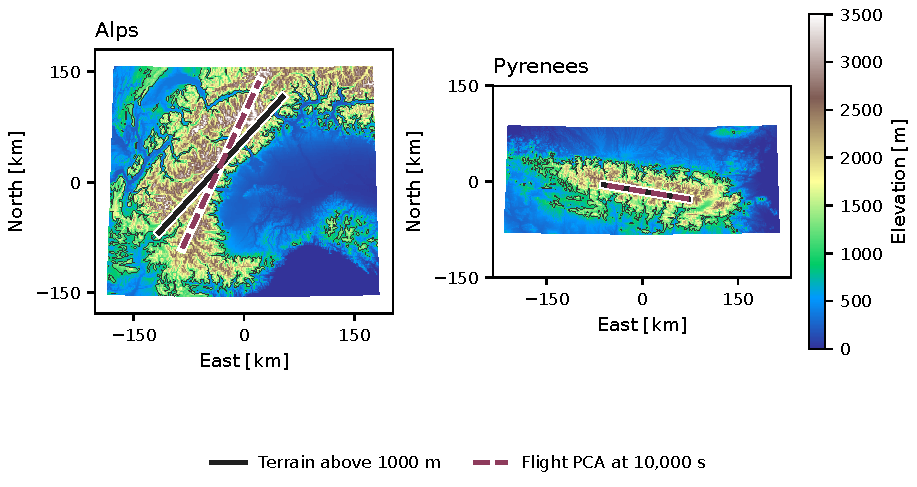
\includegraphics[width=\linewidth,height=45mm,keepaspectratio]{../thesis/generated/ch3_terrain_axes.pdf}
\takeaway{Pyrenees: separation below $1^\circ$. Alps: \StatTerrainAlpsDifference$^\circ$,
 with the flight axis more northward.}
\source{Thesis Fig. 3.22, both maps. Solid dark: terrain axis; dashed colour: flight PCA at 10,000 s. Line lengths carry no physical information.}
\question{Would terrain axes along the observed tracks explain the Alpine offset?}
\speaker{The Pyrenean comparison supports a geographical association. The Alpine chain is curved and truncated by the box. Wind, route choice and the long-flight population may also contribute. These maps use a single tangent frame per region, while flight increments use their trajectory frames and may leave the box.}
\end{frame}

\begin{frame}{Alps: shared sector, with an approximately 18-degree offset}
\begin{columns}[c,onlytextwidth]
\column{.65\textwidth}
\fig[49mm]{ch3_terrain_axis_alps.pdf}
\column{.32\textwidth}
\small
Terrain: \StatTerrainAlpsAngle$^\circ$.\par\medskip
Flight PCA: \StatTerrainAlpsFlightAngle$^\circ$.\par\medskip
Separation: \StatTerrainAlpsDifference$^\circ$.\par\medskip
\num{\StatTerrainAlpsFlights} flights support 10,000 s.
\end{columns}
\question{How much of the offset reflects Alpine curvature, box truncation or route selection?}
\source{Black: highland-footprint axis. Dashed colour: current flight PCA, shifted to the same centre. Line lengths have no physical meaning.}
\speaker{Both orientations occupy the northeast-southwest sector, but the flight covariance is more northward. A simple claim that flights run parallel to one Alpine axis misses the approximately eighteen-degree difference. The terrain angle spans 42.1 to 47.9 degrees over the three thresholds, so this sensitivity does not eliminate the offset. Wind and long-flight selection remain possible contributors; the figure neither isolates a terrain effect nor tests pilot skill.}
\end{frame}

\begin{frame}{Pyrenees: the long-lag spread follows the highland axis}
\begin{columns}[c,onlytextwidth]
\column{.65\textwidth}
\fig[49mm]{ch3_terrain_axis_pyrenees.pdf}
\column{.32\textwidth}
\small
Terrain: \StatTerrainPyreneesAngle$^\circ$.\par\medskip
Flight PCA: \StatTerrainPyreneesFlightAngle$^\circ$.\par\medskip
Separation: less than $1^\circ$.\par\medskip
\num{\StatTerrainPyreneesFlights} flights support 10,000 s.
\end{columns}
\question{Does the alignment persist for fixed flights and for terrain sampled along their routes?}
\source{ETOPO footprint above 1000 m; threshold sensitivity: \StatTerrainPyreneesMinAngle--\StatTerrainPyreneesMaxAngle$^\circ$. Decimal agreement does not imply this physical precision.}
\speaker{The near-parallel axes support a geographical association between displacement orientation and the range. They do not establish the causal contribution of terrain. Winds can align with the same range and pilots can select routes along it. The sensitivity span is not a sampling confidence interval. The comparison is made within the exact Pyrenean take-off box, but flight increments can extend beyond it.}
\end{frame}


\begin{frame}{The terrain comparison depends on the footprint definition}
\begin{center}\small
\begin{tabular}{@{}lrrr@{}}\toprule
Region & Terrain axis & Flight axis & Separation\\\midrule
Alps & \StatTerrainAlpsAngle$^\circ$ & \StatTerrainAlpsFlightAngle$^\circ$ & \StatTerrainAlpsDifference$^\circ$\\
Pyrenees & \StatTerrainPyreneesAngle$^\circ$ & \StatTerrainPyreneesFlightAngle$^\circ$ & \StatTerrainPyreneesDifference$^\circ$\\\bottomrule
\end{tabular}
\end{center}
\small Thresholds of 500, 1000 and 1500 m give:
\[
 \text{Alps: }\StatTerrainAlpsMinAngle^\circ\text{--}\StatTerrainAlpsMaxAngle^\circ,
 \qquad
 \text{Pyrenees: }\StatTerrainPyreneesMinAngle^\circ\text{--}\StatTerrainPyreneesMaxAngle^\circ.
\]
These spans measure sensitivity to the selected highland area. They are not
confidence intervals. Decimal agreement does not imply that the physical mountain
direction is known to that precision.
\source{Thesis Section 3.5.2, commentary following Fig. 3.22.}
\question{Does the comparison change with the box boundary or a local valley direction?}
\speaker{The main PCA has \StatTerrainAlpsFlights\ Alpine and \StatTerrainPyreneesFlights\ Pyrenean flights at this lag. Neither map measures the terrain exposure of individual flights.}
\end{frame}

\begin{frame}{Channel Coast: the reference height follows the PCA windows}
\begin{columns}[T,onlytextwidth]
\column{.53\textwidth}
\small
\textbf{Same population as the 10,000-s PCA}
\begin{itemize}
 \item \num{\StatWindFlights} paraglider flights.
 \item \num{\StatWindWindows} nonoverlapping windows, wholly inside retained segments.
 \item Mean cleaned GNSS altitude along each window; equal window weights.
\end{itemize}
\column{.43\textwidth}
\small
\textbf{Mean: \SI{\StatWindHeightM}{\metre}}\par\medskip
Equal flight weights: \SI{\StatWindHeightFlightM}{\metre}.\par\medskip
Middle half of window means:\\
\SI{\StatWindHeightLowM}{\metre}--\SI{\StatWindHeightHighM}{\metre}.\par\medskip
Approximate altitude above sea level; recorder datums are not harmonised.
\end{columns}
\question{Is one representative height sufficient, or should wind be matched to the altitude and location of each flight window?}
\source{Trapezoidal integration on the same 10-s segment grids. The target describes the supported long-lag windows; it is not take-off altitude or height above the terrain.}
\speaker{The mean is 1006.262 metres across 2013 exact PCA windows from 1680 flights, with the same equal-window weighting as the covariance. Each window altitude is a trapezoidal time average of cleaned GNSS z interpolated onto the existing 10-second grid. No gap is bridged. Equal weight per contributing flight gives 980.260 metres; the window-mean quartiles are 853.932 and 1159.549 metres. Short flights do not define this target because they cannot contribute at 10000 seconds. The raw GNSS vertical datum is not harmonised, so MSL is an approximation; these numbers do not imply metre-level physical accuracy. The quartile range describes heterogeneity, not uncertainty in the mean. Matching the target height does not yet match flight dates, instantaneous positions or local atmospheric conditions.}
\end{frame}

\begin{frame}{ERA5 wind is interpolated to the measured flight altitude}
\small
\textbf{2016--2025, hourly; nine cells in the coastal box; 1000/925/850/700 hPa.}
\[
 H=\Phi/g_0,\qquad h=\frac{R_\oplus H}{R_\oplus-H},\qquad
 \theta_w=\operatorname{atan2}(\langle v(h)\rangle,\langle u(h)\rangle).
\]
Convert geopotential to each hour's level heights. Interpolate \textbf{E/N wind components} to \SI{\StatWindHeightM}{\metre}, between above-ground bounds.\par\medskip
\textbf{Main comparison: all year, all hours vs.\ all year, 09--17 UTC.}\par
April--September is a separate seasonal check. Winds at 10/100 m AGL provide lower-level controls.
\question{How much of the surface-to-flight-height contrast reflects vertical shear, season and the flight conditions represented?}
\source{\href{https://doi.org/10.24381/cds.bd0915c6}{ECMWF/Copernicus ERA5 pressure levels}, accessed through a pinned snapshot of \href{https://registry.opendata.aws/earthmover-era5/}{Earthmover's public cloud-optimised ERA5 copy on AWS}. Earthmover distributes this lossless copy; it is not a separate reanalysis. Complete hourly extract: 32.22 MB compressed, preserved in the repository and on SSD.}
\speaker{Use the same nine grid cells as the surface analysis: latitudes 48.75, 49.75, 50.75 degrees and longitudes minus 1.25, zero, 1.25 degrees. Geopotential height is Phi divided by 9.80665; geometric height uses spherical Earth radius 6371000 metres. A pressure level changes altitude from hour to hour. Linear interpolation acts on eastward and northward velocities, never direction angles. All 789048 cell-hour profiles bracket the main target above the model surface. Average components over time and with cosine-latitude cell weights, then reduce the towards-angle modulo 180 degrees for comparison with PCA. The annual all-hour selection has 87672 hours per cell; 09 through 17 UTC inclusive has 32877. The two warm-season selections have 43920 and 16470. UTC is fixed, without a daylight-saving correction. Source values, timestamps, coordinates, pressure levels, geopotential, surface geopotential and hashes are preserved losslessly for offline reuse.}
\end{frame}

\begin{frame}{At flight height, both annual references remain offset from PCA}
\centering\fig[52mm]{ch3_channel_wind.pdf}
\takeaway{Annual gaps at flight height: \StatWindHeightAllDifference$^\circ$ for all hours, \StatWindHeightDayDifference$^\circ$ for 09--17 UTC.}
\question{Why is the seasonal contrast larger near the surface?}
\source{Thesis Fig. 3.23, complete figure. Angles counterclockwise from east. The rose shows where air moves towards at \SI{\StatWindHeightM}{\metre}; the black line is the \StatWindFlightAngle$^\circ$ centred PCA axis.}
\speaker{At the mean flight altitude the all-year all-hour axis is 15.8 degrees and the 09--17 UTC axis is 17.9 degrees, against 30.2 degrees for flight PCA. The corresponding separations are 14.4 and 12.3 degrees. At 10/100 metres AGL the annual axes lie closer to PCA, but their warm-daytime references rotate further away. At flight altitude the warm-daytime axis is 20.6 degrees, giving a smaller 9.6-degree separation. The altitude-matched comparison therefore has a less close annual alignment and a smaller time-selection sensitivity than the surface comparison. These are descriptive contrasts, not formal tests of different angles. The rose uses weighted 15-degree sectors, excludes speeds below 0.5 m/s only from frequencies, and retains all hours in vector means. Teal is all-year all hours; plum is all-year daytime. Green appears only in the right-hand seasonal check.}
\end{frame}

\begin{frame}{Height and time checks preserve a broad orientation resemblance}
\small
\begin{center}
\begin{tabular}{@{}lrrr@{}}\toprule
At \SI{\StatWindHeightM}{\metre} & Wind axis & PCA gap & $\rho_w$\\\midrule
All year, all hours & \StatWindHeightAllAngle$^\circ$ & \StatWindHeightAllDifference$^\circ$ & \StatWindHeightAllResultant\\
All year, 09--17 UTC & \StatWindHeightDayAngle$^\circ$ & \StatWindHeightDayDifference$^\circ$ & \StatWindHeightDayResultant\\
Apr--Sep, all hours & \StatWindHeightWarmAllAngle$^\circ$ & \StatWindHeightWarmAllDifference$^\circ$ & \StatWindHeightWarmAllResultant\\
Apr--Sep, 09--17 UTC & \StatWindHeightWarmDayAngle$^\circ$ & \StatWindHeightWarmDayDifference$^\circ$ & \StatWindHeightWarmDayResultant\\\bottomrule
\end{tabular}
\end{center}
At the quartile heights, annual axes span \StatWindSensitivityAllLowAngle--\StatWindSensitivityAllHighAngle$^\circ$ (all hours) and \StatWindSensitivityDayLowAngle--\StatWindSensitivityDayHighAngle$^\circ$ (daytime), on shared support.
\question{Does the remaining offset reflect flight selection and route choices, or change when weather is matched to actual flights?}
\source{$\rho_w=\|\langle\mathbf w\rangle\|/\langle\|\mathbf w\|\rangle$ measures cancellation. Height ranges are sensitivities, not confidence intervals. The main estimates retain all selected hours.}
\speaker{The annual all-hour and daytime resultant fractions are 0.43 and 0.44; warm-season values are 0.35 and 0.37. These do not give confidence in a direction or the fraction of observations near it. At the lower quartile height, 868 profiles at one cell have no above-ground pressure level below the target. For the height sensitivity only, exclude these 868 hours from all nine cells at every tested height, including the mean-height reference: 86804 common hours remain per cell. Apply the same seasonal and daytime masks afterward. On common support the annual quartile-height axes range from 14.3 to 17.2 degrees for all hours and from 16.4 to 19.3 degrees for daytime. Equal-flight mean altitude changes the matched reference by less than 0.3 degrees, and common-hour selection changes the main annual reference by less than 0.1 degrees. These checks retain the offset but do not calibrate receiver datums or establish significance.}
\end{frame}

\begin{frame}{What the environmental comparisons establish}
\small
\begin{tabular}{@{}p{2cm}p{10.8cm}@{}}\toprule
Region & Conclusion supported by this comparison\\\midrule
Pyrenees & Close terrain--flight alignment; a geographical association worth testing along tracks.\\[2mm]
Alps & Same broad sector, with an approximately 18-degree offset from the mean highland axis.\\[2mm]
Channel Coast & Wind at mean flight altitude lies about 12--14 degrees from PCA in both annual time selections; seasonal checks retain a broad resemblance.\\\bottomrule
\end{tabular}\par\medskip
A common constant wind shifts the mean displacement by $\tau\mathbf w$; centring removes it. Variable winds and route responses can still shape covariance.
\question{Match flight times, heights and routes to wind and local terrain before attributing the ellipse or equipment contrasts to a cause.}
\source{Independent regional references constrain an interpretation. They do not separate wind, terrain, route choice and long-flight selection.}
\speaker{The PCA concerns centred displacement spread, whereas the wind reference concerns a mean velocity. Their orientation resemblance alone cannot show that mean wind causes covariance anisotropy. Constant additive drift cancels when displacement is centred at fixed lag. Variable drift between flights, time-varying forcing and route decisions can alter covariance; their contributions need matched observations. The Pyrenean agreement is the strongest geographical alignment here. The coastal comparison at mean flight altitude retains a broadly similar sector across the four time selections, with offsets of about 10 to 14 degrees. Surface winds exhibit a larger seasonal change, so their annual near alignment should not be transferred to flight altitude. Equipment class is not measured pilot expertise, and this comparison cannot establish resistance to wind.}
\end{frame}

\begin{frame}{Reading the height labels and the mean wind}
\small
\textbf{MSL proxy}: the recorded GNSS altitude is treated approximately as altitude
above mean sea level; receiver datums have not been harmonised.
\par\medskip
\textbf{AGL}: 10 and 100 m above the ERA5 model surface. These are lower-level
wind controls, with a different vertical reference.
\[
 \rho_w=\frac{\|\langle\mathbf w\rangle\|}{\langle\|\mathbf w\|\rangle}.
\]
$\rho_w=1$ means no directional cancellation; opposite winds can give a small
resultant even when their individual speeds are large. Annual values of
\StatWindHeightAllResultant\ and \StatWindHeightDayResultant\ indicate substantial cancellation.
\source{Thesis Section 3.5.2, coastal wind reference. $\rho_w$ is not an angular confidence level.}
\question{Would flight-matched wind directions differ from the climatological vector mean?}
\speaker{Interpolate and average east/north wind components, then calculate the angle. The climatology is not paired with each flight date or instantaneous altitude. The height sensitivity checks preserve the annual offset; they do not calibrate GNSS datums.}
\end{frame}

\section{Terrain, equipment and wind}
\subsectionframe{3.5.3}{Terrain, equipment and wind}

\begin{frame}{Position, velocity and acceleration have different imbalances}
\begin{columns}[c,onlytextwidth]
\column{.56\textwidth}
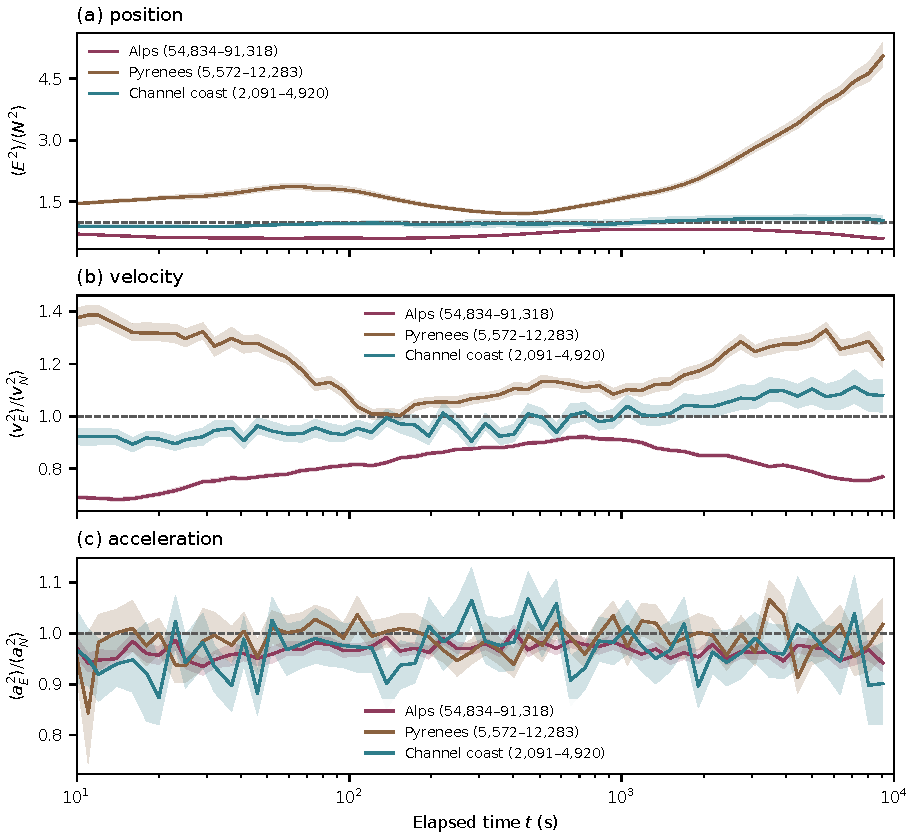
\includegraphics[width=\linewidth,height=56mm,keepaspectratio]{../thesis/generated/kinematic_isotropy_terrain.pdf}
\column{.41\textwidth}\small
All three panels use raw east/north second moments at time since launch.
\par\medskip
Median position / velocity ratios:\par
Alps: \StatKinTerrainAlpsPositionMedian\ / \StatKinTerrainAlpsVelocityMedian.\par
Pyrenees: \StatKinTerrainPyreneesPositionMedian\ / \StatKinTerrainPyreneesVelocityMedian.
\par\medskip
The Pyrenean east--west preference is consistent with terrain influencing headings;
wind and route selection remain possible contributors.
\end{columns}
\source{Thesis Fig. 3.24, all three panels, including acceleration. Shading: pointwise 10--90\% site--day bootstrap ranges.}
\question{Which directional differences persist after comparing the same sites, dates and flight durations?}
\speaker{Each panel has its own vertical range. These plots fit no scaling exponent. A ratio close to one leaves cross moments and the angular law untested.}
\end{frame}

\begin{frame}{Regional position moments differ along east and north}
\centering\fig[46mm]{terrain-position.pdf}
\takeaway{The Pyrenean position ratio rises above five at late times. The Alpine curve stays below one; the coast lies closer to one.}
\source{Thesis Fig. 3.24(a), enlarged original panel.}
\question{How much imbalance reflects mean drift, route orientation or changing support?}
\speaker{The clock is time since estimated launch, not an increment lag. Position ratios approach five in the Pyrenees. Raw second moments include both covariance and the squared mean. Splits prevent cross-gap stencils but recorded endpoint offsets can still affect these launch-referenced coordinates.}
\end{frame}

\begin{frame}{Regional velocity moments show a related directional contrast}
\centering\fig[46mm]{terrain-velocity.pdf}
\takeaway{East--west preference is also visible in Pyrenean velocity moments. The relative spread varies less than the position ratio.}
\source{Thesis Fig. 3.24(b), enlarged original panel.}
\question{Which position and velocity contrasts persist under matched conditions?}
\speaker{The regional figure pools paired east/north observations at each elapsed time and uses site-day pointwise bands. Terrain, weather, routes and the disappearing short-flight population can all contribute. Coordinate-moment balance is weaker than full isotropy.}
\end{frame}


\begin{frame}{Regional acceleration ratios are closer to unity}
\centering\fig[47mm]{section35-acceleration.pdf}
\takeaway{Acceleration has more balanced coordinate moments than the large
position contrasts. Spatially varying wind can still contribute.}
\source{Thesis Fig. 3.24(c), original panel. This is a ratio of raw second moments.}
\question{How much of this balance comes from manoeuvres, route mixing or wind gradients?}
\speaker{The acceleration ratio is approximately one in the three groups, but equal east and north moments do not establish isotropy of the acceleration distribution. Differentiation only removes a constant additive wind.}
\end{frame}

\begin{frame}{Equipment contrasts differ between the three regions}
\begin{columns}[c,onlytextwidth]
\column{.57\textwidth}
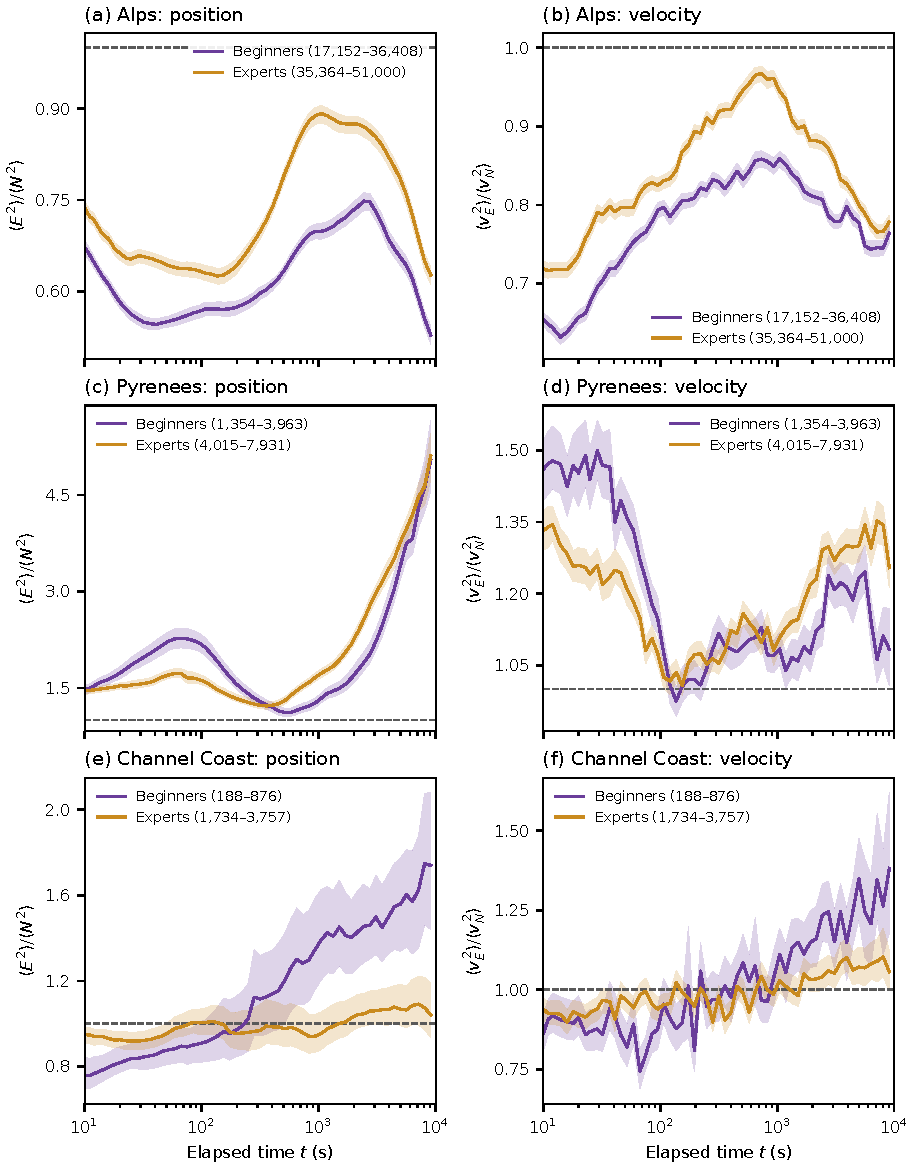
\includegraphics[width=\linewidth,height=57mm,keepaspectratio]{../thesis/generated/kinematic_isotropy_terrain_level.pdf}
\column{.40\textwidth}\small
Violet: EN A/B.\par
Ochre: EN C/D/CCC.\par\medskip
The legend uses these equipment groups as beginners/experts proxies.
\par\medskip
Actual pilot skill is unmeasured. Tandem, non-certified and unclassified records
are excluded.
\end{columns}
\source{Thesis Fig. 3.25, all six panels. The next slides enlarge each original row.}
\speaker{Certification describes tested flight behaviour and associated pilot requirements. It is not itself an aerodynamic performance ranking. An experienced pilot may fly an A/B wing.}
\end{frame}

\begin{frame}{Alps: C/D/CCC has smaller coordinate-moment imbalance}
\centering\fig[43mm]{equipment-alps-both.pdf}
\takeaway{C/D/CCC stays closer to unity over the supported times.
 Median position ratio: \StatKinTerrainAlpsEquipmentCDCCCPositionMedian,
 versus \StatKinTerrainAlpsEquipmentABPositionMedian\ for A/B.}
\source{Thesis Fig. 3.25, Alpine row.}
\question{Does the ordering persist after matching site, day, task and duration?}
\speaker{The fresh Alpine position and velocity ratios stay closer to unity for C/D/CCC over the supported grid. This is a descriptive ensemble observation. It does not establish individual isotropy, greater skill or a causal equipment effect. Violet: A/B; ochre: C/D/CCC. Beginners and experts in the retained figure legend denote equipment proxies. Bands are pointwise 10--90-percent site-day bootstrap ranges, not intervals for the group difference.}
\end{frame}

\begin{frame}{Pyrenees: the ordering of the two groups reverses}
\centering\fig[43mm]{equipment-pyrenees-both.pdf}
\takeaway{Neither group remains uniformly closer to one. Near 9086 s, position ratios are about 5.05 for A/B and 5.11 for C/D/CCC.}
\source{Thesis Fig. 3.25, Pyrenean row.}
\question{What changes between the early and later portions of the curves?}
\speaker{The Pyrenean curves do not support a uniform expert-proxy advantage. At late times both position ratios exceed five, while the velocity ordering also changes. Adjacent plotted times are correlated observations, not independent tests. Violet: A/B; ochre: C/D/CCC. Beginners and experts in the retained figure legend denote equipment proxies. Bands are pointwise 10--90-percent site-day bootstrap ranges, not intervals for the group difference.}
\end{frame}

\begin{frame}{Channel Coast: the late position contrast is pronounced}
\centering\fig[43mm]{equipment-coast-both.pdf}
\takeaway{Near 9086 s: 1.74 for A/B and 1.04 for C/D/CCC, with 188 and 1733 contributing flights.}
\source{Thesis Fig. 3.25, coastal row.}
\question{Can matching conditions separate directional route choice from wind response?}
\speaker{Near 9086 seconds the position ratios are about 1.74 for A/B and 1.04 for C/D/CCC, supported by 188 and 1733 paired flights. These are raw ensemble second moments and the samples differ strongly. Coastal cliffs and valleys prevent a wind-only interpretation. Violet: A/B; ochre: C/D/CCC. Beginners and experts in the retained figure legend denote equipment proxies. Bands are pointwise 10--90-percent site-day bootstrap ranges, not intervals for the group difference.}
\end{frame}

\begin{frame}{Two additional regions extend the coastal comparison}
\begin{columns}[c,onlytextwidth]
\column{.57\textwidth}
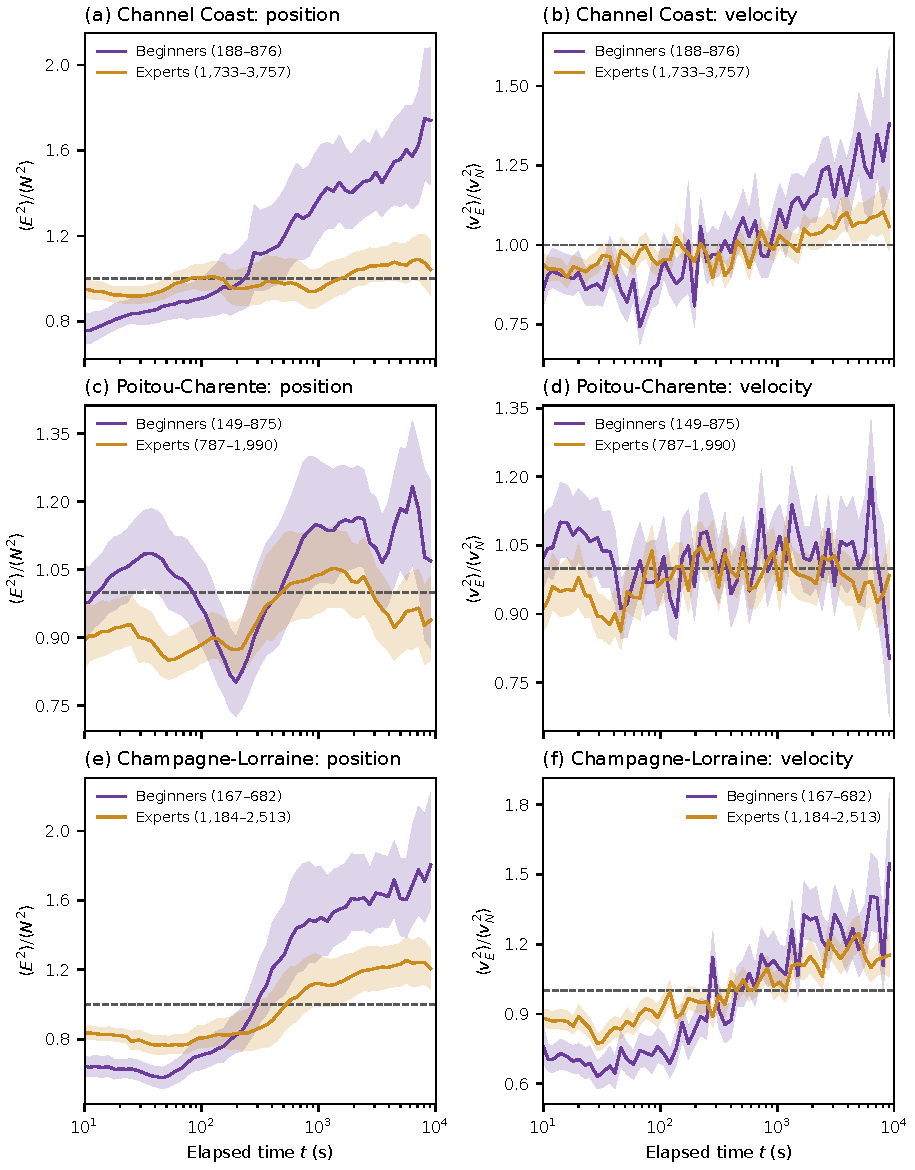
\includegraphics[width=\linewidth,height=57mm,keepaspectratio]{../thesis/generated/kinematic_isotropy_flat_level.pdf}
\column{.40\textwidth}\small
The coastal row is repeated to compare it directly with Poitou-Charente and
Champagne-Lorraine.
\par\medskip
These boxes classify take-offs. They do not measure the terrain crossed by each
flight or ensure that the equipment groups experienced comparable weather.
\end{columns}
\source{Thesis Fig. 3.26, all six panels.}
\question{Does the coastal pattern persist in other regions and on matched flight conditions?}
\speaker{The boxes are broad geographic selections, not verified polygons of flat terrain. The following two slides enlarge the additional regions. The coastal row is the same comparison shown in Fig. 3.25.}
\end{frame}

\begin{frame}{Poitou-Charente: the group curves cross}
\centering\fig[43mm]{equipment-poitou-both.pdf}
\takeaway{The curves cross and their bands overlap broadly. A consistent equipment ordering is not supported.}
\source{Thesis Fig. 3.26, middle row.}
\question{Does this low-relief launch box reproduce the coastal observation?}
\speaker{The crossing curves and broad overlapping bands do not support a general group ordering. These broad launch-location boxes are neither DEM-verified plains nor controls matched on weather. Violet: A/B; ochre: C/D/CCC. Beginners and experts in the retained figure legend denote equipment proxies. Bands are pointwise 10--90-percent site-day bootstrap ranges, not intervals for the group difference.}
\end{frame}

\begin{frame}{Champagne-Lorraine: a late contrast does not keep C/D/CCC at unity}
\centering\fig[43mm]{equipment-champagne-both.pdf}
\takeaway{A late position contrast appears, but the C/D/CCC ratio also rises above one.}
\source{Thesis Fig. 3.26, bottom row.}
\question{Which parts of the coastal hypothesis transfer to this separate region?}
\speaker{A later position contrast appears, but the C/D/CCC ratio also rises above one. Region, route mixture, weather and declining support must be separated before claiming the same physical cause. Violet: A/B; ochre: C/D/CCC. Beginners and experts in the retained figure legend denote equipment proxies. Bands are pointwise 10--90-percent site-day bootstrap ranges, not intervals for the group difference.}
\end{frame}

\begin{frame}{The environmental interpretation remains a hypothesis}
\small
\textbf{Hypothesis to discuss}\par
Equipment and pilot choices may moderate directional constraints associated with
wind and terrain. Similar mountain profiles may reflect shared route constraints.
\par\medskip
\textbf{Evidence limiting that interpretation}\par
The Pyrenean ordering reverses; class is an experience proxy; coastal terrain is
not absent; late support differs; and ensemble balance does not establish
individual isotropy or performance.
\question{What observation would distinguish this hypothesis from different sites, tasks, weather or route mixtures?}
\speaker{Preserve the proposed explanation as a useful hypothesis rather than silently removing it or presenting it as established. Similar curve shape does not by itself establish a common cause or an unavoidable terrain constraint. Wind and terrain can interact, so the coast/mountains split does not identify their separate effects.}
\end{frame}

\begin{frame}{Equal east and north moments do not establish isotropy}
\[
 \rho_{EN}=1,\qquad
 \Sigma=\begin{pmatrix}1&0.9\\0.9&1\end{pmatrix},\qquad
 \lambda_1/\lambda_2=19.
\]
\small This centred Gaussian has balanced coordinate moments but strongly unequal
principal variances.
\par\medskip
A pooled mixture of east-directed and north-directed routes can also balance the
ensemble while each flight remains directional.
\question{Are we observing mean drift, centred directional variability, or a mixture of individually oriented routes?}
\speaker{Full isotropy requires rotation invariance of the law. An isotropic covariance alone would still be only a second-order condition. Raw moments additionally contain the outer product of the mean with itself. An intentional downwind route can be successful despite being directional, so this ratio is not a direct performance score.}
\end{frame}

\begin{frame}{Coastal flights still encounter terrain and selection effects}
\small
The Channel Coast includes cliffs and valleys, including the Pays de Caux.
Wind and terrain may jointly orient lift and routes.
\par\medskip
Equipment groups can differ in sites, weather, task and duration. Their bootstrap
bands reflect one grouping structure; the groups have not been meteorologically
matched.
\par\medskip
Poitou-Charente and Champagne-Lorraine do not reproduce a uniform
C/D/CCC advantage. The coastal observation alone does not establish a general
flatland mechanism.
\source{Thesis Section 3.5.3, Equipment, terrain and selection.}
\question{Does the contrast survive when both equipment groups are observed on the same site--days?}
\speaker{Similar mountain curve shapes can suggest shared constraints but cannot identify a common cause. Wind and terrain interact. Equipment, pilot choice and task remain entangled.}
\end{frame}

\begin{frame}{Ground velocity combines air-relative motion and wind}
\[
 \mathbf v_{\mathrm{ground}}=\mathbf v_{\mathrm{air}}+\mathbf w_h.
\]
\small For a wind field $\mathbf w_h(\mathbf r,z,t)$,
\[
 \mathbf a_{\mathrm{ground}}
 =\frac{\mathrm d\mathbf v_{\mathrm{air}}}{\mathrm dt}
 +\partial_t\mathbf w_h
 +(\mathbf v_{\mathrm{ground}}\cdot\nabla_h)\mathbf w_h
 +\dot z\,\partial_z\mathbf w_h.
\]
A constant additive wind disappears under differentiation. A steady wind field
can still affect acceleration when the glider crosses horizontal or vertical gradients.
\source{Thesis Section 3.5.3, Wind and ground velocity.}
\question{Which wind contribution can be estimated independently along the tracks?}
\speaker{Ground velocity alone cannot separate still-air motion from wind. Mean route choice and net progress also affect the observed trajectories. Randomly rotating flights preserves their radii and provides an alignment control, without recovering air-relative motion.}
\end{frame}

\begin{frame}{Compare equipment groups under similar flight conditions}
\small
\begin{enumerate}
 \item Restrict comparisons to shared take-off sites and days, with comparable
 flight duration and task.
 \item Separate mean ground drift, centred spread and individual route directions.
 \item Match wind to flight times and heights, and terrain to the actual tracks.
 \item Where possible, compare the same pilot using different wings.
\end{enumerate}
Upwind progress, air-relative performance and choice of route are different
outcomes. The equipment interpretation depends on which one is being tested.
\source{Thesis Section 3.5.3, Discriminating comparisons.}
\question{Which comparison can most directly distinguish route selection from an equipment effect?}
\speaker{Thermal-centre drift may supply an independent wind estimate after segmentation, subject to assumptions about thermal motion. Site--day bootstrap estimates uncertainty; matching addresses comparability.}
\end{frame}
\end{document}
